\documentclass[a4paper,12pt]{article}
\usepackage{listing}
\usepackage{graphicx}

\begin{document}
    
\title{Multi User Chat Server}
\author{Santhisenan A}
\date{\today}
\maketitle
    
\section{Socket programming}
    
% \subsection{some title here}
Sockets can be thought of as endpoints in a communication channel that is 
bi-directional, and establishes communication between a server and one or 
more clients. Here, we set up a socket on each end and allow a client to interact 
with other clients via the server. The socket on the server side associates itself 
with some hardware port on the server side. Any client that has a socket associated
with the same port can communicate with the server socket.
    
\section{Multi-Threading}



A thread is sub process that runs a set of commands individually of any other thread.
So, every time a user connects to the server, a separate thread is created for that user
and communication from server to client takes place along individual threads based on
socket objects created for the sake of identity of each client.
We will require two scripts to establish this chat room. One to keep the serving running,
and another that every client should run in order to connect to the server.

\section{Server Side Script}
The server side script will attempt to establish a socket and bind it to an IP address and port specified by the user (windows users might have to make an exception for the specified port number in their firewall settings, or can rather use a port that is already open). The script will then stay open and receive connection requests, and will append respective socket objects to a list to keep track of active connections. Every time a user connects,
a separate thread will be created for that user. In each thread, the server awaits a message, and sends that message to other users currently on the chat. If the server encounters an error while trying to receive a message from a particular thread, it will exit that thread.

\section{Code}
\subsection{Server}
\begin{verbatim}
    # server for chat room using tcp

import socket 
import select # to provide accessto the select() and poll() functions available in most operating systems
import sys # system specific parameters and function
from thread import * # provides low-level primitives for working with multiple threads

server = socket.socket(socket.AF_INET, socket.SOCK_STREAM) # server socket in tcp
server.setsockopt(socket.SOL_SOCKET, socket.SO_REUSEADDR, 1) 


IP_ADDR = "127.0.0.1"
PORT = 8000 
server.bind((IP_ADDR, PORT))

server.listen(100)

clients = [] # list of clients


def remove(connection):
    if connection in clients:
        clients.remove(connection)

def broadcast(message, connection):
    for client in clients:
        if client != connection:
            try:
                client.send(message)
                break
            except:
                client.close()
                
                remove(client)


def clientThread(conn, addr):
    conn.sendto("Hi there, ~from server..!", addr)

    while True:
        try:
            message = conn.recv(2048)
            if message:
                print "[" + addr[0] + "]: "+ str(addr[1]) + " => "+ message
                broadcastMessage = "<[" + addr[0] + "] :" + str(addr[1]) + "> => "+ message
                broadcast(broadcastMessage, conn)
            else: 
                remove(conn)
        except: 
            continue


while True:
    conn, addr = server.accept()
    clients.append(conn)
    print addr[0] + ":"+ str(addr[1])+ " connected"
    start_new_thread(clientThread,(conn,addr)) 
conn.close()
server.close()                               

\end{verbatim}

\subsection{Client}

\begin{verbatim}
# client for chat room
import socket
import select
import sys

server = socket.socket(socket.AF_INET, socket.SOCK_STREAM)


IP_ADDRESS = "127.0.0.1"
PORT = 8000
server.connect((IP_ADDRESS, PORT))

while True:
    sockets = [sys.stdin, server]
    read_sockets, write_socket, error_socket = select.select(sockets,[],[])
    for sock in read_sockets:
        if sock == server:
            message = sock.recv(2048)
            print message
        else:
            message = sys.stdin.readline()
            server.send(message)
            sys.stdout.write("<You>")
            sys.stdout.write(message)
            sys.stdout.flush()
server.close()                    

\end{verbatim}
 
\section{Output}
\pagebreak

\begin{figure}
	
\includegraphics[width=\linewidth]{./server-chat.png}
	\caption{Client}
	\label{fig:client}
\end{figure}

\begin{figure}
	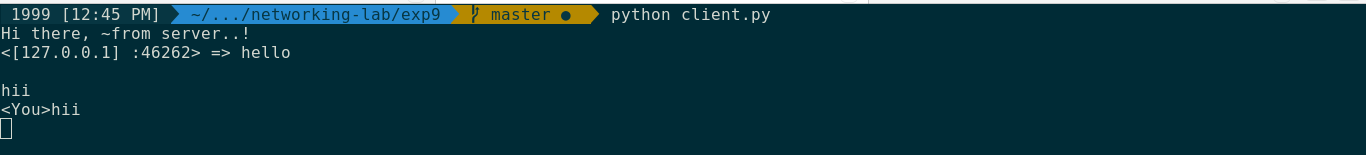
\includegraphics[width=\linewidth]{./client-1.png}
	\caption{Client}
	\label{fig:client}
\end{figure}

\begin{figure}
	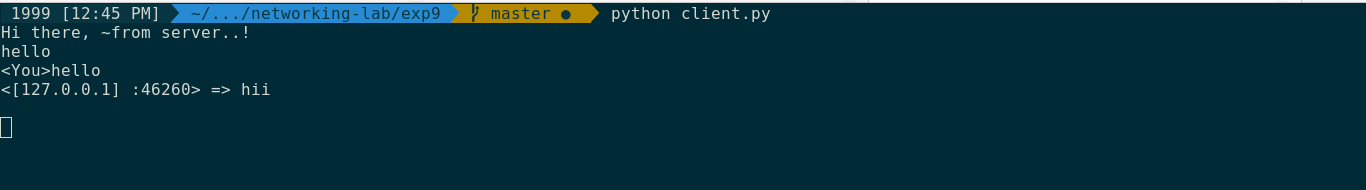
\includegraphics[width=\linewidth]{./client-2.png}
	\caption{Client}
	\label{fig:client}
\end{figure}


\end{document}